\ifx\wholebook\relax\else
\input{../Common.tex}
\input{../macroes.tex}
\begin{document}
\fi

\project
\chapter{Advanced L-Systems as Objects}\label{ch:lsystem2}

\begin{chapterfigure}
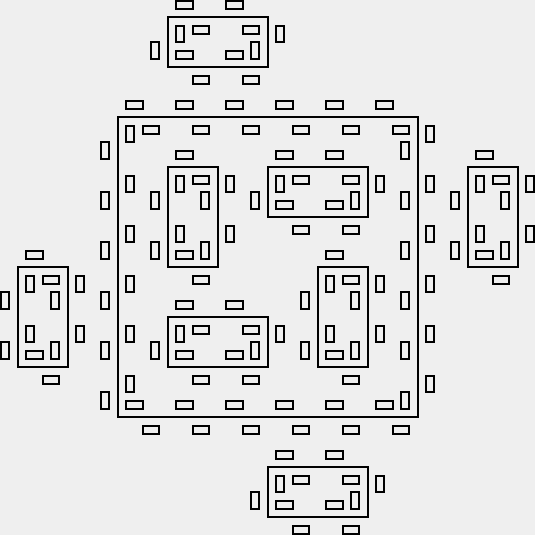
\includegraphics{island}
\end{chapterfigure}

In the previous chapter we proposed you to program the simplest form
of L-Systems. We also discussed the proposed solution and explained
why this solution was not elegant. In this chapter we propose you to
implement more complex L-Systems that can contain multiple rules and
subfigures. The resulting implementation is reused in the next chapter
in which we extend it to simulate plant growth.

\section{Modeling L-Systems with Objects}
The first implementation of an L-System was extremely simple and
consisted of small number of methods. We already explained that the
major drawback of this implementation,  besides its intrinsic limitation,
is that some methods that we defined in the class \ct{Turtle} have nothing
to do with a turtle. This is a clear sign that our design of L-System
was not well designed.

As we already mentioned in chapter~ref{}, one of the major
difficulties while programming with an object language is to identify
the right objects and the way they collaborate. A good heuristic to
follow is that objects should have a \emph{limited} set of
\emph{clearly defined responsibilities and collaborators} with
which they interact.

There is no unique way to implement a given problem, that's why
practionners and researchers developed \emph{methodologies} to help
identifying objects and developing applications. The one we prefer is
responsibilities driven design \cite{Wirf90} and is based on the use
of CRC (Class Responsibility Collaborators) cards \cite{CRC}.  The
idea is to identify for each class, its responsibilities and
collaborators and be able to write all these information on small
cards. If a single card is not enough then this is the sign that your
class is doing too much. Then we also like to take one problem at a
time without thinking too much in advance for all the possible
extensions that the system may have to take into account.  Some other
methodologies try to cover all the possible extensions of an
application in advances which may work for well-defined domain and non
changing mind customers. In this book we chose an incremental approach
where we implement the objects when they are needed.  Note that
finding the right methodology to develop object-oriented systems is
and will continue to stay a hot debate between methodologists and
practionners themselves.


\subsection{Three classes}
In the case of L-Systems we identify three kinds of objects: the
\ct{LSystem} class, the \ct{Rule} class and the \ct{Turtle} class. Figure
~\ref{fig:relLSystem} describes the relationships between these classes. 

\begin{description}
\item{The class \ct{LSystem} and its responsibilities.} It 
represents an L-System, i.e., an axiom and a set of rules. An L-System
knows how to derive itself from an axiom and a set of production
rules.  An L-System is composed by rules and collaborates with a
turtle that interprets graphically its production.

\item{The class \ct{Rule} and its responsibilities.} It represents a rule that 
composes an L-System.  A rule is composed by a left part and a right
part. A rule knows if it matches a given information. Additional
information such conditions that have to hold to apply the rule may
also be represented by this class or subclasses.

\item{The class \ct{Turtle} and its responsibilities.} It represents a sowftare turtle. It can be enhanced to know how to make drawing from different information. 
\end{description}

In fact the class \ct{Rule} is not absoluletely necessary. There are
ways (like using a dictionary or hash table whose keys represent the
left parts and values the right part of rules) to implement the simple
rules directly into the class \ct{LSystem}. However, we decided to
define an explicit class \ct{Rule} because it is an important entity
of the \ct{LSystem} domain. Moreover, we wanted to implement specific
methods like printing to help you debugging and as you will see
in chapter~\ref{ch:parametric} parametric L-Systems requires more
complex rules.

\begin{figure}[!htbp]
\centerline{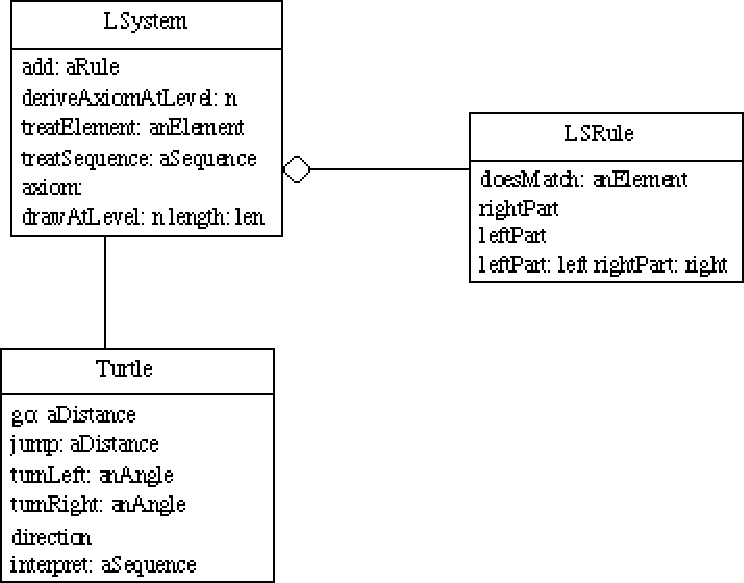
\includegraphics[width=10cm]{relLSystem}}
\caption{Relationships between the different classes participating in the L-System application. (For the Reviewers: we will explain somewhere the meaning of the signs.}
\label{fig:relLSystem}
\end{figure}



\paragraph{An Example.} The following script shows the creation of an 
L-System representing the fibonacci suite shown in~\ref{sec:lsystem}
and how its derivation can be invoked. The lengths of each production
iterations constitutes the Fibonacci suite (1, 1, 2, 3, 5, 8...).

\begin{scriptwithtitle}{LSystem representing Fibonacci Suite}\label{scr:fibo}
LSystem class>>fibonacci
   "self fibonacci"

   | lsys |
   lsys := LSystem  new axiom: 'B'.
   lsys add: (LSRule leftPart: 'B' rightPart: 'A').
   lsys add: (LSRule leftPart: 'A' rightPart: 'AB').
   ^lsys deriveAxiomAtLevel: 4
\end{scriptwithtitle}

After declaring a variable, a new \ct{LSystem} instance is created,
the axiom \ct{'B'}, a string, is specified. Then two rules are created
and added to the L-System. Finally, the L-System is asked to produce
and return the production for the fourth iteration.  A rule is
composed by a string representing the left part and a string
representing the right part (See~\ref{sec:stringascol}).

\paragraph{Preparing.} Before defining the corresponding classes, 
open a new project named L-System, this will allow you to save all the
changes you will do in one file and to browse the changes you will
perform. Then open a browser and define a new category
\index{category} named L-System in which we will define all the
classes relative to L-System.


\section{The \ct{Rule} class}\label{sec:ruleclass}
The behavior of a rule should allow us to specify the left and right
parts of a rule, to test if a given element of a derivation match the
rule and to print a rule so that we can understand them more easily.

\paragraph{Do it.} Define the class \ct{LSRule} that inherits from the 
class \ct{Object}. We suffix the name of the class by \ct{LS} to avoid
name problems\footnote{Namespaces have been introduced in other
Smalltalks and it may happen that namespaces will be introduced in
Squeak too.}, it may happen that somebody else already used such a
name for another class. To represent the left and right part of a rule
you can choose to use two named instance variables named for example
\ct{leftPart} and \ct{rightPart}.  Define the accessors for these two instances
variables.

\hidden{
\begin{classdef}
Object subclass: #LSRule
	instanceVariableNames: 'leftPart rightPart '
	classVariableNames: ''
	poolDictionaries: ''
	category: 'L-System'
\end{classdef}}

\subsection{Interface for Instance Creation} 
As there is no real sense to create a rule without specifying the left
part and the right part, define the \emph{class} method in the
'instance creation' protocol named \ct{leftPart:rightPart:} that
creates a rule and initializes it with the arguments passed as shown
by the following script.

\begin{scriptwithouttitle}
LSRule leftPart: 'A' rightPart: 'AB'
\end{scriptwithouttitle}


\paragraph{Deeper: Discussions about Creation Responsibility.}
Note that by proposing an interface for the creation of instance you,
as responsible of the class, control that the created instance is
well-formed. Different degrees of control can be applied. For example, if you
do not want to allow the creation of instance via the class method \ct{new} you can 
override it to raise an error this way: 

\begin{method}
LSRule class>>new
   
   self error: 'To create an instance of ', 
               self name, 
               ' you should use leftPart:rightPart'.
\end{method}

However, you may notice that this choice implies that you cannot
invoke anymore the method \ct{new} in the class method
\ct{leftPart:rightPart:} via \ct{self}. The best way to solve this problem is  to invoke the method \ct{basicNew} to create a non-initialize instance
as shown by the following method. Note that method starting with
\ct{basic} should never be overriden to be sure that we can always
invoke them.

\begin{method}
LSRule class>>leftPart: left rightPart: right

  ^ self basicNew leftPart: left ; rightPart: right
\end{method}

Another non elegant way to solve this problem would have been to
invoke \ct{new} via the \ct{super} instance variable. We strongly
discourage you to do so because you would unnecessary coupled classes.
This is a good guidelines to only use \ct{super} to invoke a method
with the same selector that the one containing the \ct{super}.


\subsection{Rule Behavior}
Having well formed rules was the first step. The second step is to be
able to know if a given rule can be applied, i.e., if we can
substitute the left part by its right part while doing the axiom
derivation. This is definitively a responsibility of a rule, so
implement the method \ct{doesMatch: anElement} that returns true if a
rule matches a given element.

\begin{scriptwithouttitle}
| r1 |
r1 := LSRule leftPart: 'A' rightPart: 'AB'.
r1 doesMatch: 'B'.
\emph{returns false}
r1 doesMatch: 'A'
\emph{returns true}
\end{scriptwithouttitle}

The implementation of \ct{doesMatch:} is really simple. This
simplicity is not a problem! What is important to realize is that this
rule behavior could be much more complex and that providing a method
for it allow us to change it without disturbing the other classes using rules.

\paragraph{Adapted Printing.} In Smalltalk, any object can return a string 
representing it.  This is really useful while developing an
application. This behavior is specified by the methods
\ct{printOn:}. Look for all the  implementors of \ct{printOn:} to see how the system uses this functionality.  

By default the system proposes a generic mechanism to print any
object, read the code of the method \ct{printOn:} defined on the class \ct{Object}. However, using such a generic printing mechanism does not provide a lot of information. 

For example printing (via the Print It menu) the following expression
which could contain more information.
\begin{scriptwithouttitle}
LSRule leftPart: 'A' rightPart: 'AB'
\emph{displays the string a LSRule} 
\end{scriptwithouttitle}

Redefine the method \ct{printOn:} in the category 'printing' as follow: 

\begin{method}
LSRule>>printOn: aStream

   aStream nextPutAll: 'Rule: '.
   aStream nextPutAll: leftPart.
   aStream nextPutAll: ' -> '.
   aStream nextPutAll: rightPart
\end{method}

Once this method is defined, printing the previous rule displays the
following text: \ct{Rule: B -> AB} which conveys much more information. 

\begin{scriptwithouttitle}
LSRule leftPart: 'A' rightPart: 'AB'
\emph{displays the string Rule B -> AB} 
\end{scriptwithouttitle}


\begin{figure}[!htbp]
\centerline{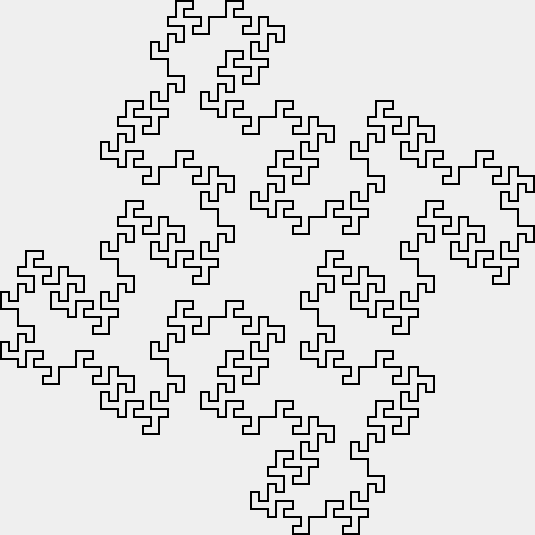
\includegraphics[width=10cm]{quadraKoch}}
\caption{n = 2, angle = 90, Axiom: \emph{F-F-F-F}, \emph{F $\rightarrow$ F+FF-FF-F-F+FF-F-F+F+FF+FF-F}}
\label{fig:quadraKoch}
\end{figure}


\section{The L-System class}
An L-System object contains the following information: its axiom and a
set of production rules. From a behavioral perspective, an L-System
should provides fonctionality to define such information but more
importantly how to derive the axiom using the rules.


\subsection{Class definition and Instance Initialization.} 
Define the class \ct{LSystem} that inherits from \ct{Object} in the
\ct{'L-System'} class category. This class should have two instance
variables named for example, \ct{axiom} and \ct{rules} to represent
the axiom and the set of rules.  The definition of such a class is
shown below:

\begin{classdef}
Object subclass: #LSystem
   instanceVariableNames: 'rules axiom'
   classVariableNames: ''
   poolDictionaries: ''
   category: 'L-System'
\end{classdef}

Create a category \ct{'accessing'} and define the accessors relative
to the \ct{axiom} instance variable.

\paragraph{Instance Variable Initialization.} As explained 
in~\ref{sec:variableinitialization}, specialize the class method
\ct{new} to invoke automatically the method \ct{initialize} on any newly
created instances and to return it.

To represent a set of rule we can different data structures like a set
(only one element and no order) , a bag (multiple occurences of the
same element and no order) an array (indexed by integers and not
growing), an ordered collection (ordered but growing), dictionary
(indexed by a hash function and growing). 

As the order of the rules is irrelevant, we chose to use a set to hold
the collection of rules. Define the method \ct{initialize} in the
category \ct{'initialize'} so that the default value of the \ct{axiom}
instance variable is an empty string (\ct{''}) and the value of the
\ct{rules} instance variable is a \ct{Set} instance.

In the category \ct{'rule addition'}, define the method \ct{add:} that
add a given rule to the set of rules used by the L-System. Hints: Look
for information in the class \ct{Collection} and its subclasses.

\subsection{Deeper: Discussions about Set and Identity} 
A set does not allow to contain twice the same object.  This leads to
asking the question of object identity. By default, a set uses the
hash value of the object to check if the object can be added to
itself. As we did not redefine the hash value of rule, two instances
representing the \emph{same} rule are in fact two different objects,
hence they are added to the set. In our current implementation this is
absolutely not a problem. If you want to try, define the following
method and inspect the result of the method comment.

\begin{method}
LSystem class>>twiceSameRuleAdded
   "self twiceSameRuleAdded"

   | lsys |
   lsys := self new. 
   lsys add: (LSRule leftPart: 'A' rightPart: 'AB').
   lsys add: (LSRule leftPart: 'A' rightPart: 'AB').
   ^ lsys 
\end{method}

If we would need to avoid such a kind of situation, we should do the
following: (1) redefine the \ct{=} method of the objects to represent
the equality function for the object, and (2) redefine the \ct{hash}
method to return a different hash number for the object. As both
functions are somehow related we apply the following pattern
suggested by Beck in \cite{Beck97a} in the case of a rule.  

\forreviewers{Is there any better way to write that?}

\begin{method}
LSRule>>= aRule 
   (aRule isKindOf: self class) ifFalse: [^false].
   ^ (self leftPart = aRule leftPart) and: [self rightPart = aRule rightPart]
\end{method}

\begin{method}
LSRule>>hash
   ^ self hash leftPart hash bitXor: self rightPart hash
\end{method}

The method \ct{=} is redefined: it checks if the class of the argument
is the same as or a subclass of the class of the receiver if this is
true, the left and right part should be equals too. The \ct{hash}
method is then redefine to combine the hash values of the left and
right parts. Check by inspecting the value returned by \ct{LSystem
twiceSameRuleAdded}.


\subsection{Axiom Derivation}
Deriving the axiom a given number of times is the core behavior of an
L-System. We propose you to implement it as three methods:
\ct{deriveAxiomAtLevel:}, \ct{treatSequence:}, and
\ct{treatElement:}.  \ct{deriveAxiomAtLevel:} applies a certain number
of times the rules. It does it by invoking several times the method
\ct{treatSequence:} on its own result. \ct{treatSequence:} applies the 
rules on each of the elements contained in the collection passed by
calling the \ct{treatElement:} and returns it
result. \ct{treatElement:} checks whether a rule can be applied for a
given element, if so it returns the right part of the rule, else the
right part.  

All the examples illustrating these three methods are shown in the
context of the L-System defined in~\scriptref{scr:fibo}.  So define it
as a class method of the class \ct{LSystem} in category
\ct{'examples'} as shown in \methodref{met:fibo}. Note that this way you will be able to save this
specific LSystem together with the code that implements the \ct{LSystem}
class.

\begin{method}\label{met:fibo}
LSystem class>>fibonacci
   "self fibonacci"

   | lsys |
   lsys := LSystem  new axiom: 'B'.
   lsys add: (LSRule leftPart: 'B' rightPart: 'A').
   lsys add: (LSRule leftPart: 'A' rightPart: 'AB').
   ^lsys deriveAxiomAtLevel: 4
\end{method}


\paragraph{treatElement: anElement} checks whether one of the 
rules matches the passed element. If this is the case it returns the
left part of the rule else it returns the element converted as a
string. The fact that the method always returns the same kind of
objects, here a string, is really important, this way the calling
method can use the result in an uniform manner.

\begin{scriptwithouttitle}
| fib |
fib := LSystem fibonacci.
fib treatElement: \$B.
\emph{returns 'A'}
fib treatElement: \$A.
\emph{returns 'AB'}
fib treatElement: \$C.
\emph{returns 'C'}
\end{scriptwithouttitle}

The method \ct{treatElement:} is called by the method
\ct{treatSequence:} over each element of the axiom (and the next
result of the rule application) which are strings. As a string is a
collection of characters, the element passed to \ct{treatElement:} is a
character.

\paragraph{Hints.} Look in the \ct{Collection} class for 
the method \ct{detect: aBlock ifNone: exceptionBlock} whose behavior
is explained by the following script.

\begin{scriptwithouttitle}
| col |
col := #(a 1 b 2 true).
col detect: [:each | each isNumber] ifNone: [nil].
\emph{returns 1}
col detect: [:each | each isPoint] ifNone: [nil].
\emph{returns nil}
\end{scriptwithouttitle}

\hidden{
\begin{method}
LSystem>>treatElement: aCharacter
   "returns the right part of a rule corresponding to the element 
    (aString) passed in argument "

   |rule|
   rule := rules detect: [:each | each doesMatch: aCharacter asString]
                 ifNone: [nil].
   ^ rule isNil 
       ifTrue: [aCharacter asString]
       ifFalse: [rule rightPart]
\end{method}}


\paragraph{\ct{treatSequence: aString}} invokes the method \ct{treatElement:} on 
each of the characters contained in the argument, \ct{aString} and
returns a string in which all the results have been concatenated. The
following script shows some results obtained when invoking this
method.

\begin{scriptwithouttitle}
| fib |
fib := LSystem fibonacci.
fib treatSequence: 'A'.
\emph{returns 'AB'}
fib treatSequence: 'C'.
\emph{returns 'C'}
fib treatSequence: 'ABC'
\emph{returns 'ABAC'}
fib treatSequence: 'ABCA'
\emph{returns 'ABAABABA'}
\end{scriptwithouttitle}

\paragraph{Hints.} Use the method finder to identify the method that given 
two strings returns the string representing the concatenation of them.
Then one way could be to define a local variable representing the
result of the method, then to initialize with an empty
string and to concatenate the results returned by the method
\ct{treatElement:} to this variable.

\hidden{
\begin{method}
LSystem>>treatSequence: aString 
   "Apply the rules to each element and return a string 
   that represents the result"

   | resString |
   resString := ''.
   aString do: [:aChar | resString := resString , (self treatElement: aChar)].
   ^ resString
\end{method}
}

\paragraph{\ct{deriveAxiomAtLevel: aNumber}} derives the axiom by applying
the rules a certain number of times. As we shown in the previous
chapter in section~\ref{sec:lsystem}, the derivation at a level n is
the result of the application of the rules on the axiom derivation at
level n-1.  For example, the 4 th axiom derivation results from the
rule application on the 3rd axiom derivation.

Note it is somehow similar to the method
\ct{deriveAxiom:withRule:give:atLevel:} defined in the
previous chapter.

\begin{scriptwithouttitle}
| fib |
fib := LSystem fibonacci. 
fib deriveAxiomAtLevel: 1
\emph{returns 'A'}
self deriveAxiomAtLevel: 2
\emph{returns 'AB'}
self deriveAxiomAtLevel: 3
\emph{returns 'ABA'}
self deriveAxiomAtLevel: 5
\emph{returns 'ABAABABA'}
\end{scriptwithouttitle}

\hidden{
\begin{method}
deriveAxiomAtLevel: n 
   "self new deriveAxiomAtLevel: 1"
   
   | production |
   production := axiom.
   n timesRepeat: [production := self treatSequence: production].
   ^ production
\end{method}}

\subsection{Discussion about Object-Oriented Modeling}
We would like to stress that defining the axiom derivation as the
behavior of the L-System object is what distinguish object programming
from procedural programming. In procedural programming, some data
structures representing the rules and an L-System would have been
defined and some procedures would have accessed them to derive the
axiom. Here, the key point is that the structure is only accessible by
the L-System itself. Each class defines the structure that it
manipulates, it controls the access to such information and specifies
the behavior that can be invoked to manipulate these data. Moreover,
the class with its structure and behavior is a single entity.  Note
that the internal representation of an L-System is not relevant
because as a client we are only interested by the behavior of an
L-System, i.e., the specification of the system and the axiom
derivation.


\subsection{Invoking the Graphical Interpretation}
Define the method \ct{drawAtLevel:length:angle:}. Such a method should
create a turtle and ask it to interpret (using the method
\ct{interpret:length:angle:}) the result of the method
\ct{deriveAxiomAtLevel:}.


\hidden{
\begin{method}
drawAtLevel: n length: len angle: angle

   | turtle derivation |
   turtle := TurtleWithMemory new.
   derivation := (self deriveAxiomAtLevel: n).
   turtle north;
      interpret: derivation
      length: len
      angle: angle.
   ^ derivation
\end{method}}


\section{Examples}
Now you have all the pieces of the puzzle and are in position to play with the L-Systems. First start to express all the L-Systems shown in the
previous chapter with the new way of implementing L-Systems. 

For example, the following method shows the implementation as class
methods the L-System shown by Figure~\ref{fig:Kocha}.  Define such
a method as class methods of \ct{LSystem} in a category 'examples'.
We chose to write this L-System as a method and not simply as a script
so that we are able to save it with the class and we do not have to
retype it again and again.

\begin{method}
LSystem class>>simpleBasicOne
   "self simpleBasicOne"
   
   | lsys |
   World clearTurtleTrails.
   lsys := self new.
   lsys axiom: 'F-F-F-F'.
   lsys add: (LSRule leftPart: 'F' rightPart: 'FF-F-F-F-F-F+F').
   lsys drawAtLevel: 4 length: 2 angle: 90.
\end{method}
	
You can be willing to define the following L-Systems as class methods.

\begin{tabbing}
\=aaa\=aaa\=aaa\=aaaaaaaaa\=aaaaaaaaa\=aaaaaaaaa\=aaaaaaaaa\=aaaaaaaaa\=aaaaaaaaa\kill
Quadratic Koch island (Figure~\ref{fig:quadraKoch})\\
\>\>\>\> \emph{Axiom} \>\>\emph{F-F-F-F}\\
\>\>\>\> \emph{Angle} \>\>90 degree\\
\>\>\>\> \emph{Rule}  \>\>\emph{F $\rightarrow$ F+FF-FF-F-F+FF-F-F+F+FF+FF-F}
\end{tabbing}



\begin{tabbing}
\=aaa\=aaa\=aaa\=aaaaaaaaa\=aaaaaaaaa\=aaaaaaaaa\=aaaaaaaaa\=aaaaaaaaa\=aaaaaaaaa\kill
Islands (Figure~\ref{fig:island})\\
\>\>\>\> \emph{Axiom} \>\>\emph{F+F+F+F}\\
\>\>\>\> \emph{Angle} \>\>90 degree\\
\>\>\>\> \emph{Rule}  \>\>\emph{f $\rightarrow$ ffffff}\\
\>\>\>\> \emph{Rule}  \>\>\emph{F $\rightarrow$ F+f-FF+F+FF+Ff+FF-f+FF-F-FF-Ff-FFF}
\end{tabbing}

\begin{figure}[!htbp]
\centerline{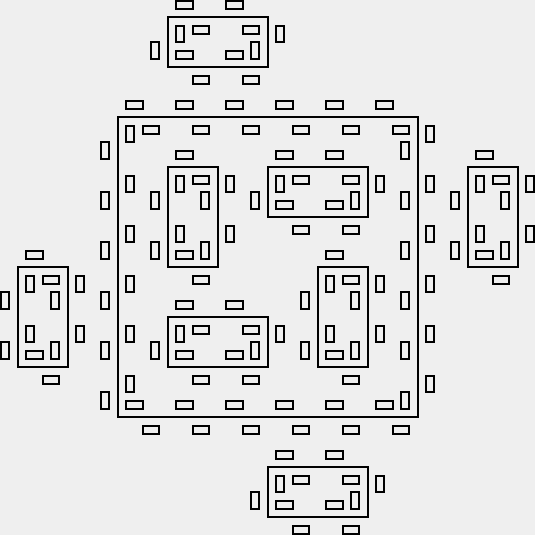
\includegraphics{island}}
\caption{Islands. n = 2, angle = 90, Axiom: \emph{F+F+F+F}, \emph{F $\rightarrow$ F+f-FF+F+FF+Ff+FF-f+FF-F-FF-Ff-FFF}, \emph{f $\rightarrow$ ffffff}}
\label{fig:island}
\end{figure}


\section{L-System containing Subfigures}

As the vocabulary that we used so far is limited to F, f, +, and -, it
is difficult to produce rich fractals, or curves whose generation is
based on multiple rules. Indeed, as the idea behind rewriting rules is
to rewrite the path followed by the turtle into subpaths, we can only
have one rule having F as left part and one rule having f.  The
L-System named Island presented in Figure~\ref{fig:island} above is
one of the rare one.  Experiment a bit to see if you can obtain nice
figures by rewriting + and -.

To solve this problem, L-Systems are simply extended to support the
definition of \emph{subfigures}. The idea is that new symbols like R
or L can appear now in the left or right part of a rule, then once the
derivation is finished the symbols are replaced by a sequence of the
original vocabulary elements, the simplest replacement being F.  The
new symbols represent simple figures that are this way repeated all
over the place. Try for example to understand figures R and L of
the Hilbert L-Systems.



The following L-System expresses the Sierpinski gasket as shown by
Figure~\ref{fig:sierpinsky}. The rules are expressed in terms of two
new symbols R and L that after the derivation are considered
equivalent to F.

\begin{tabbing}
\=aaa\=aaa\=aaa\=aaaaaaaaa\=aaaaaaaaa\=aaaaaaaaa\=aaaaaaaaa\=aaaaaaaaa\=aaaaaaaaa\kill
Sierpinski Gasket (Figure~\ref{fig:sierpinsky})\\
\>\>\>\> \emph{Axiom} \>\>\emph{R}\\
\>\>\>\> \emph{Angle} \>\>60 degree\\
\>\>\>\> \emph{Rule}  \>\>\emph{L $\rightarrow$ R+L+R}\\
\>\>\>\> \emph{Rule}  \>\>\emph{R $\rightarrow$ L-R-L}\\
\>\>\>\> \emph{Figure}  \>\>\emph{R $\rightarrow$ F}\\
\>\>\>\> \emph{Figure}  \>\>\emph{L $\rightarrow$ F}
\end{tabbing}

\begin{figure}[!htbp]
\centerline{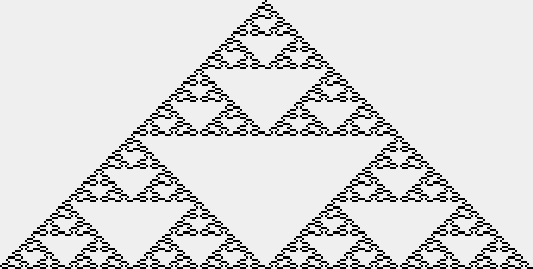
\includegraphics{sierpinsky}}
\caption{Sierpinski Gasket. n = 7, angle = 60, Axiom: \emph{R},  \emph{L $\rightarrow$ R+L+R}, \emph{R $\rightarrow$ L-R-L}, figures: \emph{L $\rightarrow$ F, R $\rightarrow$ F}.}
\label{fig:sierpinsky}
\end{figure}

The following L-System expresses the Hilbert curve. The rules are
expressed in terms of two new symbols R and L that after the
derivation are expanded into their respective definition.

\begin{tabbing}
\=aaa\=aaa\=aaa\=aaaaaaaaa\=aaaaaaaaa\=aaaaaaaaa\=aaaaaaaaa\=aaaaaaaaa\=aaaaaaaaa\kill
Hilbert Curve\\
\>\>\>\> \emph{Axiom} \>\>\emph{L}\\
\>\>\>\> \emph{Angle} \>\>90 degree\\
\>\>\>\> \emph{Rule}  \>\>\emph{L $\rightarrow$ +RF-LFL-FR+}\\
\>\>\>\> \emph{Rule}  \>\>\emph{R $\rightarrow$ -LF+RFR+FL-}\\
\>\>\>\> \emph{Figure}  \>\>\emph{R $\rightarrow$ -F+F+F-}\\
\>\>\>\> \emph{Figure}  \>\>\emph{L $\rightarrow$ +F-F-F+}
\end{tabbing}

If look at the derivation of the axiom of the Hilbert curve at level 2
before expanding figures we obtain the following result:
+-LF+RFR+FL-F-+RF-LFL-FR+F+RF-LFL-FR+-F-LF+RFR+FL-+. Then after
applying figures we get:
+-+F-F-F+F+-F+F+F-F-F+F+F-+F+F-F-F+-F-+-F+F+F-F-+F-F-F+F+F-F-F+-F-F+F+F-+F+-F+F+F-F-+F-F-F+F+F-F-F+-F-F+F+F-+-F-+F-F-F+F+-F+F+F-F-F+F+F-+F+F-F-F+-+
in which there is no symbol representing figures.




\subsection{Analysis}
From the previous examples, we see that we need:

\begin{itemize}
\item to specify that a certain element should be replaced by a 
sequence of elements representing figures. For example, in the
Hilbert curve, R has to be replaced by -F+F+F-.

\item to first derive the axiom a certain number of times and then replace the elements representing figures by their definition.
\end{itemize}

\subsection{Implementing subfigures}

We would like to have a new class to represent L-System with
subfigures because we do not want to clutter the \ct{LSystem} class
with functionality that only a subset of the L-Systems use. However,
we want to reuse the functionality defined by the class \ct{LSystem}.
So we define the new class as subclass of \ct{LSystem} and specialize
its behavior where it is needed as shown by the
Figure~\ref{fig:inhSubfigures}.

As we want to show you another way to represent simple rules
(subfigures are indeed really similar to rules), we chose not to use
the \ct{LSRule} class to represent figures but to use a
\emph{dictionary} to store the definition of figures. As an exercise
we suggest you to use rules to represent figures. So let us look at a
dictionary!


\begin{figure}[!htbp]
\centerline{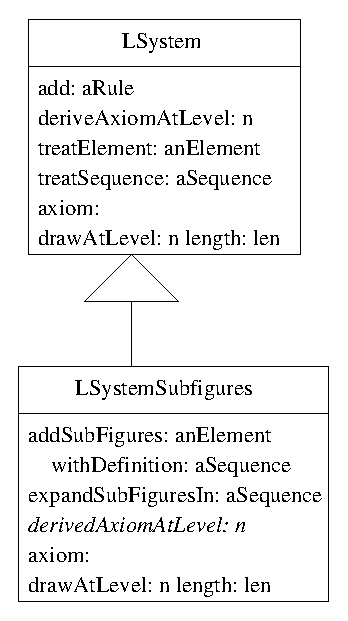
\includegraphics{inhSubfigures}}
\caption{Relationships between the different classes participating in the LSystem application. (For the Reviewers: we will explain somewhere the meaning of the signs.}
\label{fig:inhSubfigures}
\end{figure}


\paragraph{Using a Dictionary.}
A \emph{dictionary} or \emph{hash table} is a data structure that
allows one to store and access information based on keys.  It avoids
to go over long collections. Given a key and a value we can add the
value into the dictionary and later retrieve such an information by
using the associated key. The key can be any object, so it can a
symbol, a character, a string or even a turtle. The following script
shows data can be added and accessed form a dictionary.

In addition we show you some functionality that you may need for your
implementation.  It is possible to specify an action that is performed
if the key is not found in the dictionary using
\ct{at:ifAbsent:}. \ct{[nil]} is the action that returns \ct{nil}.
\ct{keys} is the message to obtain all the keys contained in a
dictionary. We suggest you to browse the class \ct{Dictionary} and try
some methods.

\begin{scriptwithouttitle}
| dict |
dict := Dictionary new.
dict at: \#caro put: Turtle new.
dict at: \#F put: 2.
dict at: 'F' put: 3.
dict at: \#caro.                    \emph{returns a turtle}
dict at: \#F.                       \emph{returns 2}
dict at: 'F'.                       \emph{returns 3}
dict at: 'A' ifAbsent: [nil].       \emph{returns nil}
dict keys.                          \emph{returns \#caro \#F \$F}
\end{scriptwithouttitle}

\subsection{An example of Subfigures}

The following method shows how the Hilbert curve L-System is defined using the class \ct{LSystemSubfigures}

\begin{method}\label{mth:hilbert}
LSystemSubFigures class>>hilbert
   "self hilbert"

   | lsys |
   lsys := self new.
   lsys axiom: 'L'.
   lsys add: (LSRule leftPart: 'L' rightPart: '+RF-LFL-FR+').
   lsys add: (LSRule leftPart: 'R' rightPart: '-LF+RFR+FL-').
   lsys addSubFigure: 'L' withDefinition: '+F-F-F+'.
   lsys addSubFigure: 'R' withDefinition: '-F+F+F-'.
   lsys drawAtLevel: 3 length: 4 angle: 90.
   ^ lsys
\end{method}

\subsection{Class Definition and Instance Initialization}
Define a class, named \ct{LSystemSubfigures}, that inherits from
\ct{LSystem} and have an instance variable that represents the
subfigures dictionary.

Define the method \ct{initialize} in the category
\ct{'initialize-release'}. Do not forget to invoke the \ct{initialize}
method defined on the superclass.

\subsection{Discussion about initialize}
The method \ct{initialize} defined on the class \ct{LSystemSubFigures}
is invoked when a new instance is created because the method \ct{new}
of the superclass invokes it. Let us analyse what's really happen!

\forreviewers{Do be done and may be moved elsewhere}

\subsection{Defining and Computing with Subfigures}
Define the method \ct{addSubFigure: aString withDefinition:
anotherString} that adds the subfigure definition as shown by the
method~\ref{mth:hilbert}. Hints: Look at \ct{Dictionary} class. 

Define the method \ct{expandSubFiguresIn: aString} that replaces in a
string all the elements representing a figure by all figure
constituants.  Here follow some tests to help you.

\begin{scriptwithouttitle}
| lsys |
lsys := LSystemSubFigures hilbert.
lsys expandSubFiguresIn: 'L'.      
\emph{returns '+F-F-F+'}
lsys expandSubFiguresIn: 'ALBL'.      
\emph{returns 'A+F-F-F+B+F-F-F+'}
lsys expandSubFiguresIn: 'AB'. 
\emph{returns 'AB'}
lsys expandSubFiguresIn: 'ALBR'. 
\emph{returns 'A+F-F-F+B-F+F+F-'}
\end{scriptwithouttitle}

\hidden{
expandSubFiguresIn: production 
   "replace all could not work"

   | subFigureCharacters col|
   subFigureCharacters := subFigures keys.
   col := OrderedCollection new.
   production do: [:each | (subFigureCharacters includes: each asString) 
	                      ifTrue: [col addAll: (subFigures at: each asString)]	                             ifFalse: [col add: each ]].
   ^ col}


Now once the axiom is derived n times we need to invoke the method
\ct{expandSubFiguresIn:}. What we need is to specify that the \ct{derivaAxiomAtLevel:} method have to execute normally and then expand figures. 
To do so we just have to redefine the method \ct{deriveAxiomAtLevel:}
on the class \ct{LSystemSubFigures} to invoke the default behavior of
this method defined on \ct{LSystem}, keep the result returned and pass
it to \ct{expandSubFiguresIn:}.

\hidden{
deriveAxiomAtLevel: n 
	| production |
	production := super deriveAxiomAtLevel: n.
	^ self expandSubFiguresIn: production
}


\subsection{Another example of L-System}

The Dragon Curve shown in Figure~\ref{fig:dragon} is a well-known
recursive curve. It can be expressed as follow:

\begin{tabbing}
\=aaa\=aaa\=aaa\=aaaaaaaaa\=aaaaaaaaa\=aaaaaaaaa\=aaaaaaaaa\=aaaaaaaaa\=aaaaaaaaa\kill
Dragon Curve (Figure~\ref{fig:dragon})\\
\>\>\>\> \emph{Axiom} \>\>\emph{L}\\
\>\>\>\> \emph{Angle} \>\>90 degree\\
\>\>\>\> \emph{Rule}  \>\>\emph{L $\rightarrow$ L+R+}\\
\>\>\>\> \emph{Rule}  \>\>\emph{R $\rightarrow$ -L-R}\\
\>\>\>\> \emph{Figure}  \>\>\emph{R $\rightarrow$ F}\\
\>\>\>\> \emph{Figure}  \>\>\emph{L $\rightarrow$ F}
\end{tabbing}

\begin{figure}[!htbp]
\centerline{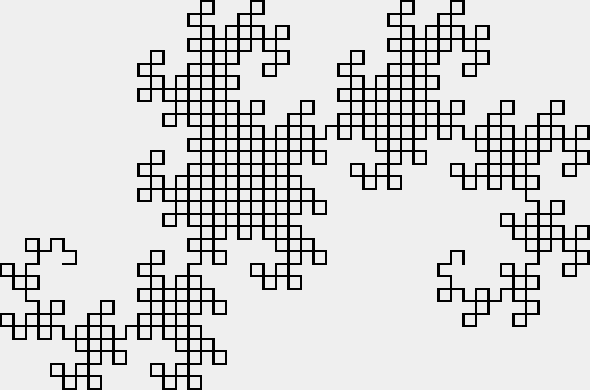
\includegraphics{dragon}}
\caption{n = 7, angle = 60, Axiom: \emph{L},  \emph{L $\rightarrow$ L+R+}, \emph{R $\rightarrow$ -L-R}, figures: \emph{L $\rightarrow$ F, R $\rightarrow$ F}.}
\label{fig:dragon}
\end{figure}



\subsection{FASS Curves}
Now you can experiment with the following LSystems that produce FASS
curves (space-Filling, self-Avoiding, simple and self-Similar). The
particularity of these definition is that the new symbols are simply
ignored. In our implementation we can replaced them by an empty
string. Note that if you implemented the 
\ct{interpret:length:angle:} method on the class \ct{Turtle} to skip 
elements not belonging to the vocabulary of the turtle you can avoid
to define such emptying figures.

\begin{figure}[!htbp]
\centerline{
\includegraphics{FASS1}}
\caption{FASS1: n = 3, length = 4}
\label{fig:Fass1}
\end{figure}


\begin{tabbing}
\=aaa\=aaa\=aaa\=aaaaaaaaa\=aaaaaaaaa\=aaaaaaaaa\=aaaaaaaaa\=aaaaaaaaa\=aaaaaaaaa\kill
FASS1 (Figure~\ref{fig:Fass1}\\
\>\>\>\> \emph{Axiom} \>\>\emph{-L}\\
\>\>\>\> \emph{Angle} \>\>90 degree\\
\>\>\>\> \emph{Rule}  \>\>\emph{L $\rightarrow$ LF+RFR+FL-F-LFLFL-FRFR+}\\
\>\>\>\> \emph{Rule}  \>\>\emph{R $\rightarrow$ -LFLF+RFRFR+F+RF-LFL-FR}\\
\>\>\>\> \emph{Figure}  \>\>\emph{R $\rightarrow$ }\\
\>\>\>\> \emph{Figure}  \>\>\emph{L $\rightarrow$ }
\end{tabbing}

\begin{figure}[!htbp]
\centerline{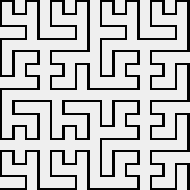
\includegraphics{FASS2}}
\caption{FASS2: n = 2, length = 6}
\label{fig:Fass2}
\end{figure}



\begin{tabbing}
\=aaa\=aaa\=aaa\=aaaaaaaaa\=aaaaaaaaa\=aaaaaaaaa\=aaaaaaaaa\=aaaaaaaaa\=aaaaaaaaa\kill
FASS2 (Figure~\ref{fig:Fass2})\\
\>\>\>\> \emph{Axiom} \>\>\emph{-L}\\
\>\>\>\> \emph{Angle} \>\>90 degree\\
\>\>\>\> \emph{Rule}  \>\>\emph{L $\rightarrow$ LFLF+RFR+FLFL-FRF-LFL-FR+F+RF-LFL-FRFRFR+}\\
\>\>\>\> \emph{Rule}  \>\>\emph{R $\rightarrow$ -LFLFLF+RFR+FL-F-LF+RFR+FLF+RFRF-LFL-FRFR}\\
\>\>\>\> \emph{Figure}  \>\>\emph{R $\rightarrow$ }\\
\>\>\>\> \emph{Figure}  \>\>\emph{L $\rightarrow$ }
\end{tabbing}

\begin{figure}[!htbp]
\centerline{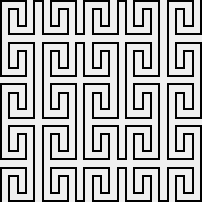
\includegraphics{FASS3}}
\caption{FASS3: n = 3, length = 2}
\label{fig:Fass3}
\end{figure}

\begin{tabbing}
\=aaa\=aaa\=aaa\=aaaaaaaaa\=aaaaaaaaa\=aaaaaaaaa\=aaaaaaaaa\=aaaaaaaaa\=aaaaaaaaa\kill
FASS3 (Figure~\ref{fig:Fass3})\\
\>\>\>\> \emph{Axiom} \>\>\emph{-L}\\
\>\>\>\> \emph{Angle} \>\>90 degree\\
\>\>\>\> \emph{Rule}  \>\>\emph{L $\rightarrow$ L+F+R-F-L+F+R-F-L-F-R+F+L-F-R-F-L+F+R-F-L-F}\\
\>\>\>\>\>\> \emph{-R-F-L+F+R+F+L+F+R-F-L+F+R+F+L-F-R+F+L+F+R-F-L+F+R-F-L}\\
\>\>\>\> \emph{Rule}  \>\>\emph{R $\rightarrow$ R-F-L+F+R-F-L+F+R+F+L-F-R+F+L+F+R-F-L+F+R+F}\\
\>\>\>\>\>\> \emph{+L+F+R-F-L-F-R-F-L+F+R-F-L-F-R+F+L-F-R-F-L+F+R-F-L+F+R}\\
\>\>\>\> \emph{Rule}  \>\>\emph{K $\rightarrow$ L+F+R-F-L+F+R-F-L-F-R+F+L-F-R-F-L+F+R-F-L-F}\\
\>\>\>\>\>\> \emph{-R-F-L+F+R+F+L+F+R-F-L+F+R+F+L-R-F+F+L+F+R-F-L+F+R-F-L}\\
\>\>\>\> \emph{Figure}  \>\>\emph{R $\rightarrow$ }\\
\>\>\>\> \emph{Figure}  \>\>\emph{L $\rightarrow$ }\\
\>\>\>\> \emph{Figure}  \>\>\emph{K $\rightarrow$ }
\end{tabbing}


\begin{figure}[!htbp]
\begin{minipage}[c]{.5\linewidth}
\centerline{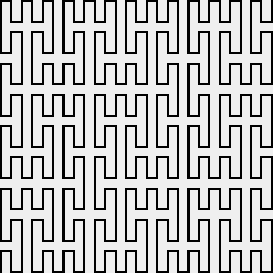
\includegraphics[width=\linewidth]{peano}}
\end{minipage}
\begin{minipage}[c]{.5\linewidth}
\centerline{
\includegraphics[width=\linewidth]{QuadraGosper}}
\end{minipage}
\caption{Peano Curve: n = 1 and Quadratic Gosper Curve: n = 2}
\label{fig:peano}
\end{figure}


\begin{tabbing}
\=aaa\=aaa\=aaa\=aaaaaaaaa\=aaaaaaaaa\=aaaaaaaaa\=aaaaaaaaa\=aaaaaaaaa\=aaaaaaaaa\kill
Peano Curve (Figure~\ref{fig:peano})\\
\>\>\>\> \emph{Axiom} \>\>\emph{S}\\
\>\>\>\> \emph{Angle} \>\>90 degree\\
\>\>\>\> \emph{Rule}  \>\>\emph{S $\rightarrow$ SFZFS+F+ZFSFZ-F-SFZFS}\\
\>\>\>\> \emph{Rule}  \>\>\emph{Z $\rightarrow$ FSFZ-F-SFZFS+F+ZFSFZ}\\
\>\>\>\> \emph{Figure}  \>\>\emph{S $\rightarrow$ F+F+F-F-F}\\
\>\>\>\> \emph{Figure}  \>\>\emph{Z $\rightarrow$ F-F-F+F+F}
\end{tabbing}

\begin{tabbing}
\=aaa\=aaa\=aaa\=aaaaaaaaa\=aaaaaaaaa\=aaaaaaaaa\=aaaaaaaaa\=aaaaaaaaa\=aaaaaaaaa\kill
Quadratic Gosper Curve (Figure~\ref{fig:peano})\\
\>\>\>\> \emph{Axiom} \>\>\emph{-R}\\
\>\>\>\> \emph{Angle} \>\>90 degree\\
\>\>\>\> \emph{Rule}  \>\>\emph{L $\rightarrow$ LL-R-R+L+L-R-RL+R+LLR-L+R+LL+R-LR-R-L+L+RR-}\\
\>\>\>\> \emph{Rule}  \>\>\emph{R $\rightarrow$ +LL-R-R+L+LR+L-RR-L-R+LRR-L-RL+L+R-R-L+L+RR}\\
\>\>\>\> \emph{Figure}  \>\>\emph{L $\rightarrow$ F}\\
\>\>\>\> \emph{Figure}  \>\>\emph{R $\rightarrow$ F}
\end{tabbing}


\begin{figure}[!htbp]
\centerline{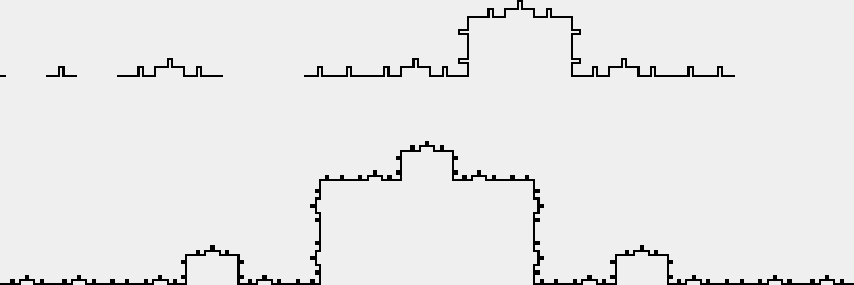
\includegraphics{alltower}}
\caption{Towers. The following curves shows the derivation of an L-System created using subfigures at level 0,1,2,3,and 4. Note that the length used is 2 pixels  except for the last one where we used 1 pixel.}
\label{fig:alltower}
\end{figure}


\begin{exonofig}
Try to define a LSystem that produces the previous picture.

\end{exonofig}
\hidden{tower
	"self tower"

	| lsys |
	lsys := self new axiom: 'F'.
	lsys add: (LSRule leftPart: 'F' rightPart: 'LF+L-F-L+FL').
	lsys add: (LSRule leftPart: 'L' rightPart: 'FF').
	lsys addSubFigure: 'L' withDefinition: 'FF'.
	World clearTurtleTrails.
	lsys drawAtLevel: 2 length: 2 angle: 90.
	^ lsys}


\section{Other Implementation Strategies}
We propose you some alternative implementation solutions.

\begin{exonofig}
Implement figures as \ct{LSRule} instances. The implementation
should be then similar to the one of plain rules.
\end{exonofig}

\begin{exonofig}
Without changing the interface of the class \ct{LSystem} (method names and
arguments) use a dictionary instead of an ordered collection to store the 
\ct{LSRule}.
\end{exonofig}

\paragraph{Using an array.} As we mentioned earlier, instead of using two instance variables for the left and right part of a rule you can also use only one instance variable holding an array. Here using an array is not a really good
idea because (1) the class definition will lose readibility, (2)
accessing one or the other parts requires an extra indirection, and
(3) the extra array created does not bring anything.

In fact, using instance variable holding an array or a collection is
definitively better suited when the size of objects held by the
collection is changing for instances to instances of the class.  This
is the case with the instance variable rules of the class
\ct{LSystem}, in such a case each L-System can have a different number
of rules.

Nevertheless, this is a good exercise for you. It shows you that the
implementation of a class can change without breaking the behavior of
such a class. This way encapsulation prevents having too much to
change when a different implementation decision is required.

Change the implementation the rule class without changing the
functionality it provides to use an array. Hints: you may pay
attention to initialize the instance variable holding the array with
an empty array of size two. Read \ref{sec:variableinitialization}.

\section{Further Readings}

\begin{description}
\item \cite{Wirf90} is a first book in the literature that presented 
the concept of responsibility driven design. It is interesting to see how from 
objects are identified from a textual description. 

\item \cite{Riel96} presents a set of heuristics to support you during the design of your application. The concepts are presented using C++, however the
heuristics are general and applicable in any object-oriented language.
\end{description}


\ifx\wholebook\relax\else\end{document}\fi
